\RequirePackage[l2tabu, orthodox]{nag}
\documentclass[12pt,a4paper]{article}
\usepackage[utf8]{inputenc} 
\usepackage[T1]{fontenc}
\usepackage[english]{babel} 
\usepackage{geometry}
\geometry{a4paper}
\usepackage{longtable}


%----------------------------KODE START---------------------------------------
\usepackage{listings}
\usepackage{color}
\usepackage[usenames,dvipsnames]{xcolor}
\usepackage{textcomp}

\definecolor{comment}{rgb}      {0.38, 0.62, 0.38}
\definecolor{keyword}{rgb}      {0.10, 0.10, 0.81}
\definecolor{identifier}{rgb}   {0.00, 0.00, 0.00}
\definecolor{string}{rgb}       {0.50, 0.50, 0.50}

\lstset
{
   language=erlang,
   % general settings
   numbers=left,
   frame=single,
   basicstyle=\footnotesize\ttfamily,
   tabsize=2,
   breaklines=true,
   showstringspaces=false,
   % syntax highlighting
   commentstyle=\color{comment},
   keywordstyle=\color{keyword},
   identifierstyle=\color{identifier},
   stringstyle=\color{string},
}
%----------------------------KODE SLUT----------------------------------------


\setlength\parindent{0pt} % Makes \noindent standard
\usepackage{graphicx} 
\usepackage{caption}
\usepackage{subcaption}
\usepackage{float} 
\usepackage{wrapfig} % Allows in-line images if needed
\usepackage{hyperref}
\usepackage{cleveref}
\usepackage{amsmath}
\usepackage{mathtools}
\hypersetup{colorlinks=false,hidelinks, citecolor=black, urlcolor=black}
\usepackage{csquotes}
\usepackage{comment}

\usepackage[dot, autosize, outputdir="dotgraphs/"]{dot2texi}
\usepackage{tikz}
\usetikzlibrary{shapes}
\usepackage{url}
\usepackage{booktabs}
\usepackage{multirow}
\usepackage{longtable}
\setcounter{secnumdepth}{4}
\setcounter{tocdepth}{4}
\usepackage[titletoc]{appendix} % Names appendices "Appendix A"
                                % instead of just A in Contents
\usepackage[bottom]{footmisc}
\usepackage{pdfpages}


%\usepackage{lmodern}
\usetikzlibrary{arrows,automata}
\usepackage{verbatim}

\linespread{1.2} 
\graphicspath{{./figures/}} 

\newcommand{\fasto}{\textsc{Fasto} }
\newcommand{\mips}{\textsc{Mips} }
\newcommand{\mars}{Mars }

%-----------------------------------------------------------------------------
% HEADER AND FOOTER STUFF
%-----------------------------------------------------------------------------
\usepackage{fancyhdr}
\usepackage{lastpage} % Making it possible to write ``Page x of y'' in the footer

\pagestyle{fancy}
\fancyhf{}
% Header stuff below
\lhead{Jenny-Margrethe Vej} 
\chead{}
\rhead{rwj935} 
% Footer stuff below
\cfoot{Page \thepage \hspace{1pt} of \pageref{LastPage}} % To the left at the bottom

%-----------------------------------------------------------------------------
\begin{document}

%\includepdf[pages={-}]{../forside_tex_ting/forside.pdf}

I here have my data from the last week - just to show my experiences. Usually the days are quite accurate, but I can definitely see something funny also... :) Oh, and yes - I am horrible at prioritising my sleep! I will try to be as honest as possible in the caption, where I shortly describes what you see. :) I have noted my self, that I am under influence of my exams (even though they are done, I have so much anxiety during exams they affects me for several weeks after) - and also I am pretty affected by the fact, I just got into a new relationship, which is of course a positive effect on my mind, but doubtless it is affecting my sleeping pattern. 

\begin{figure}[H]
    \begin{subfigure}[b]{0.5\textwidth}
        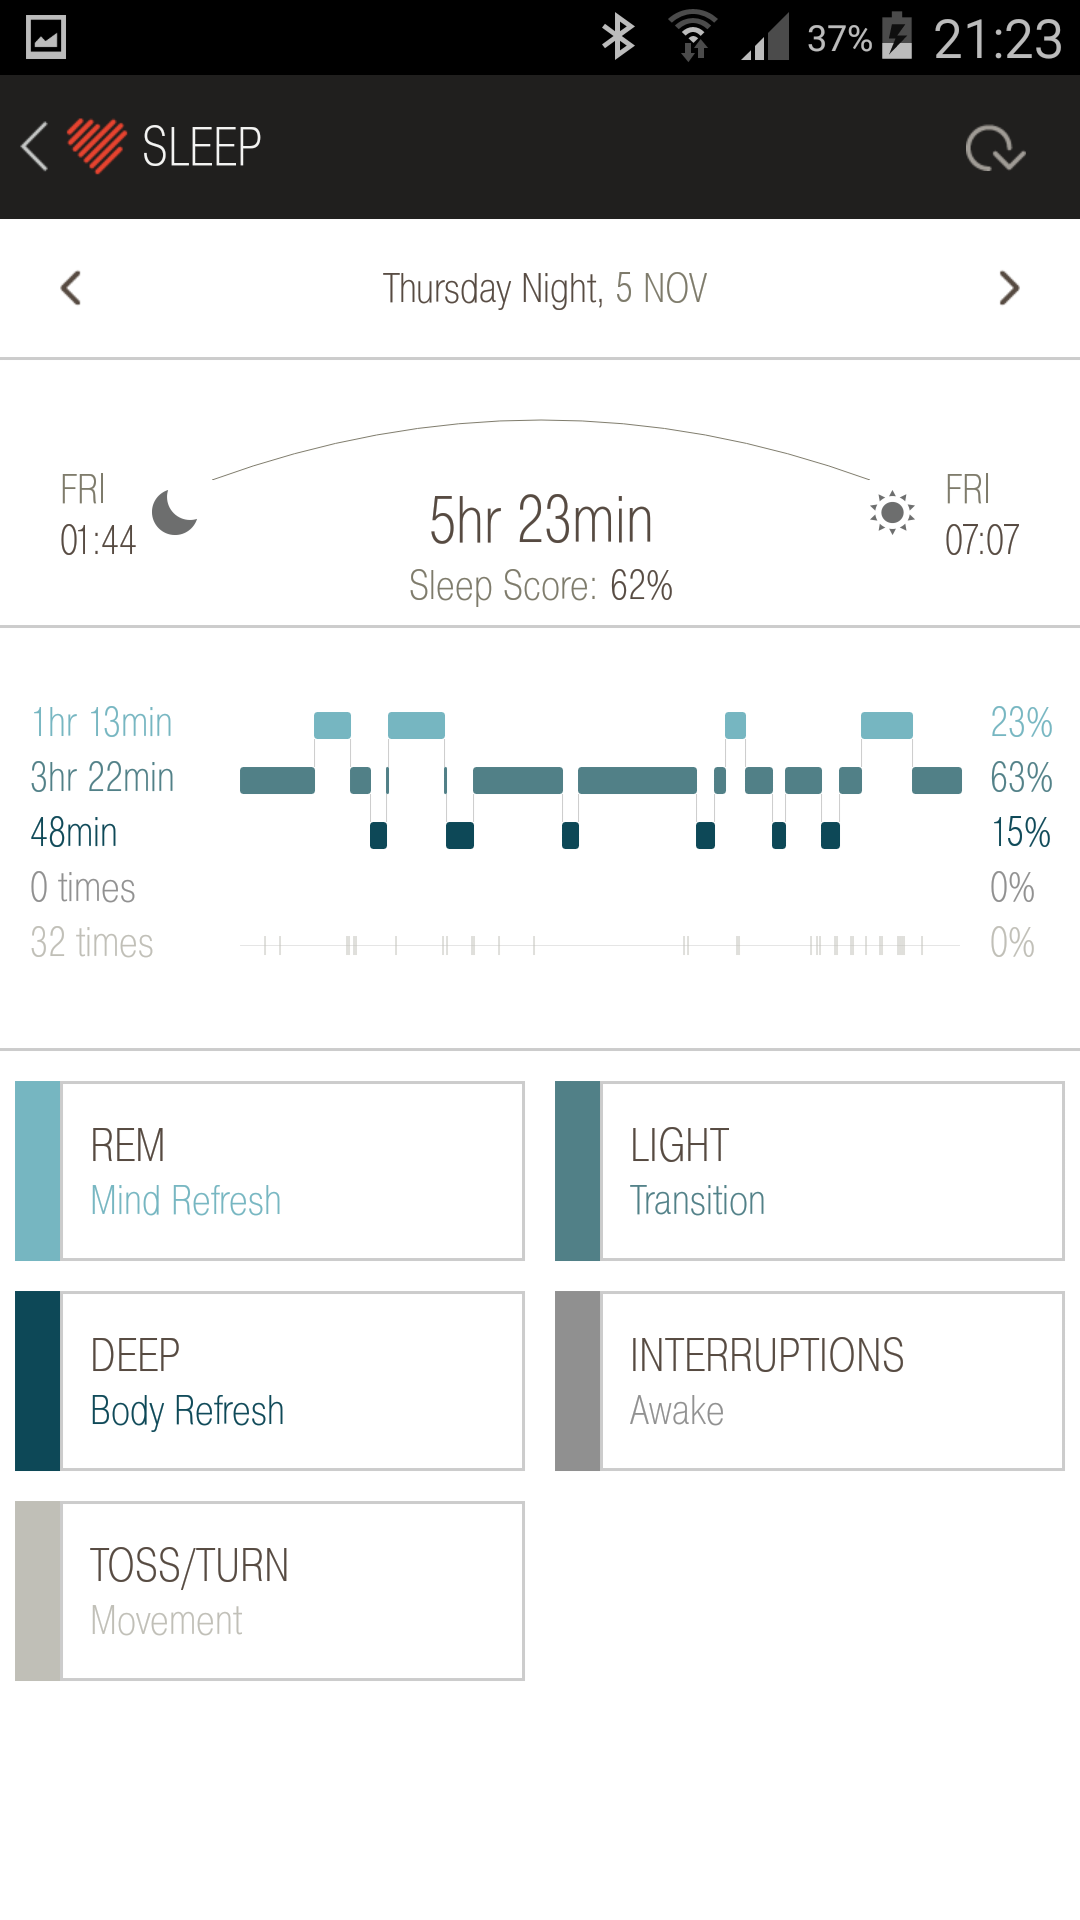
\includegraphics[width=\textwidth]{05-11-15.png}
     \end{subfigure}
    ~ %add desired spacing between images, e. g. ~, \quad, \qquad, \hfill etc. 
      %(or a blank line to force the subfigure onto a new line)
    \begin{subfigure}[b]{0.5\textwidth}
        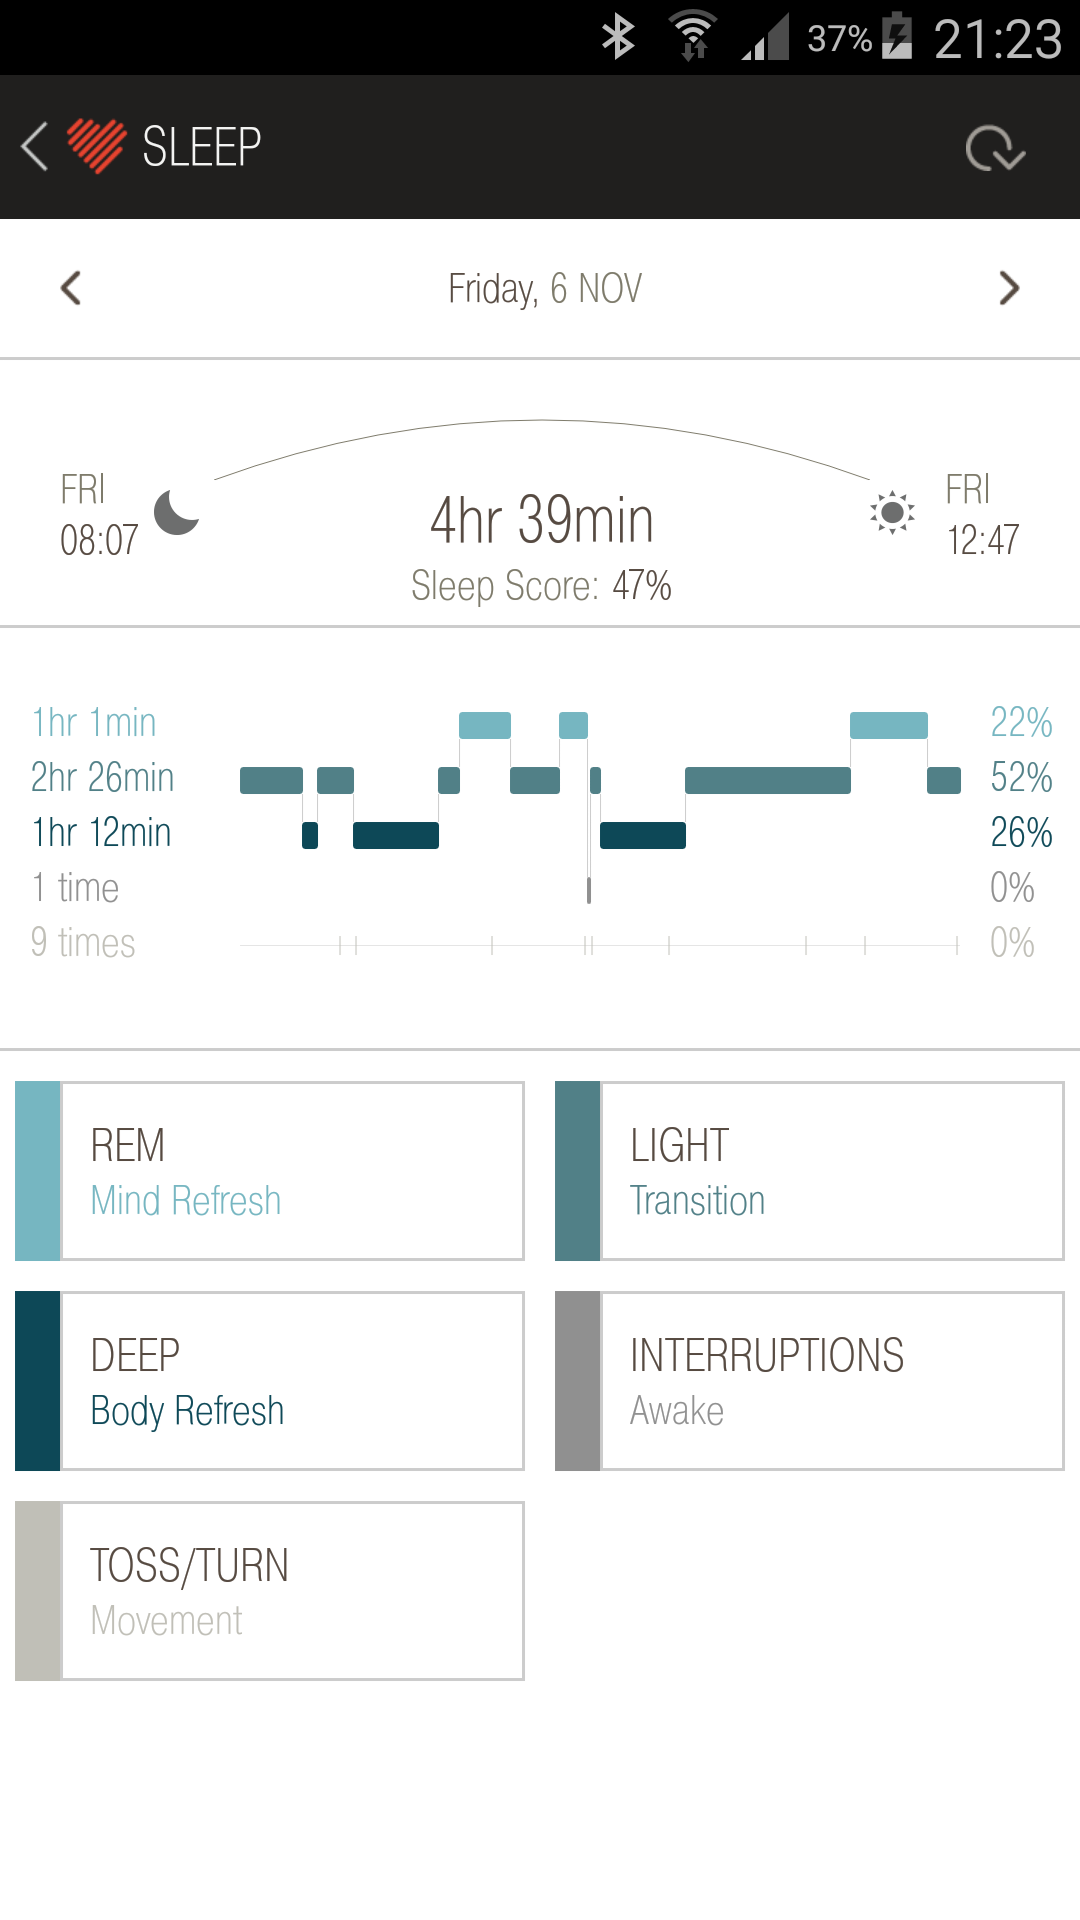
\includegraphics[width=\textwidth]{06-11-15.png}
    \end{subfigure}
\caption{Actually this is the same ``night'' - I was celebrating the end of my exam Thursday night, and got to bet around 01:44 in the night before Friday. Between 07:07 and 08:07 Friday morning something happened - and my watch decided not to measure anything	. If I check the webpage instead of the phone, the hour is just marked with diagonally gray stripes.}
\end{figure}

\newpage

\begin{figure}[H]
    \begin{subfigure}[b]{0.5\textwidth}
        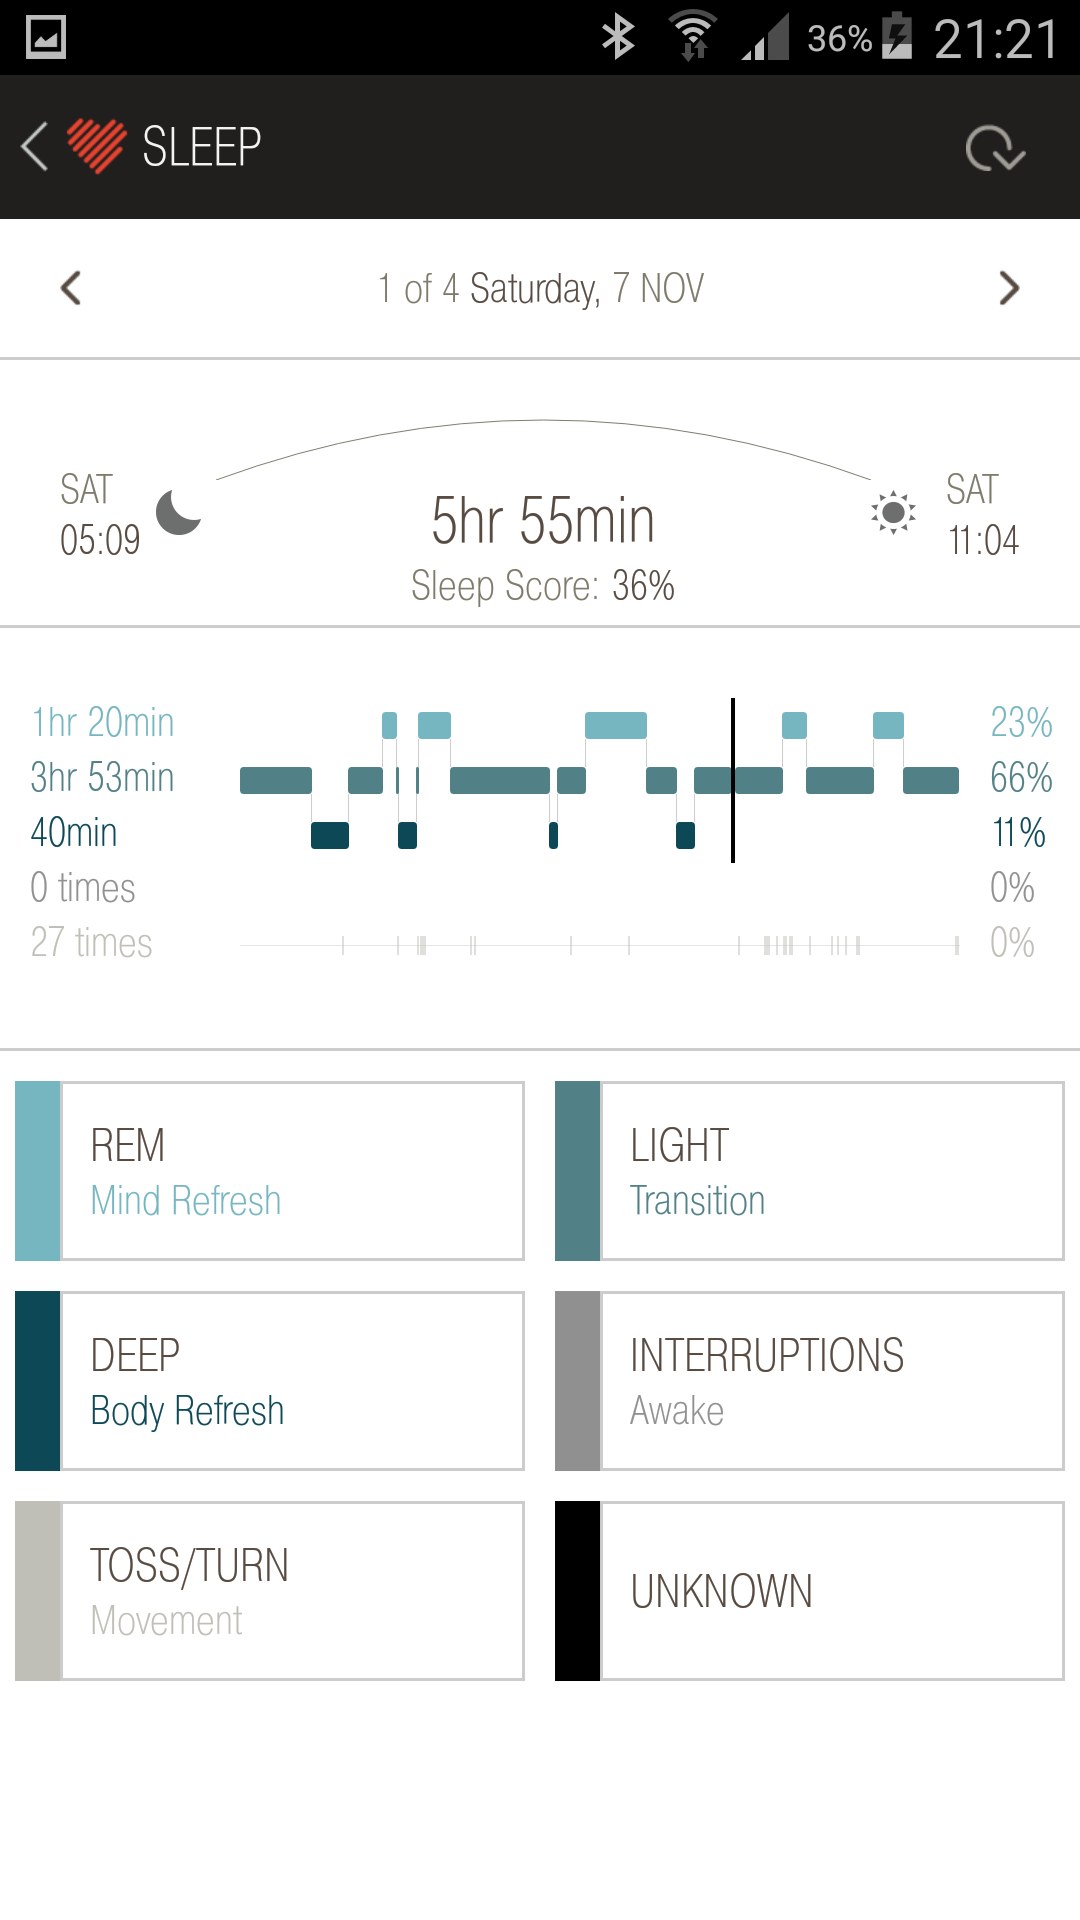
\includegraphics[width=\textwidth]{07-11-15-1.png}
     \end{subfigure}
    ~ %add desired spacing between images, e. g. ~, \quad, \qquad, \hfill etc. 
      %(or a blank line to force the subfigure onto a new line)
    \begin{subfigure}[b]{0.5\textwidth}
        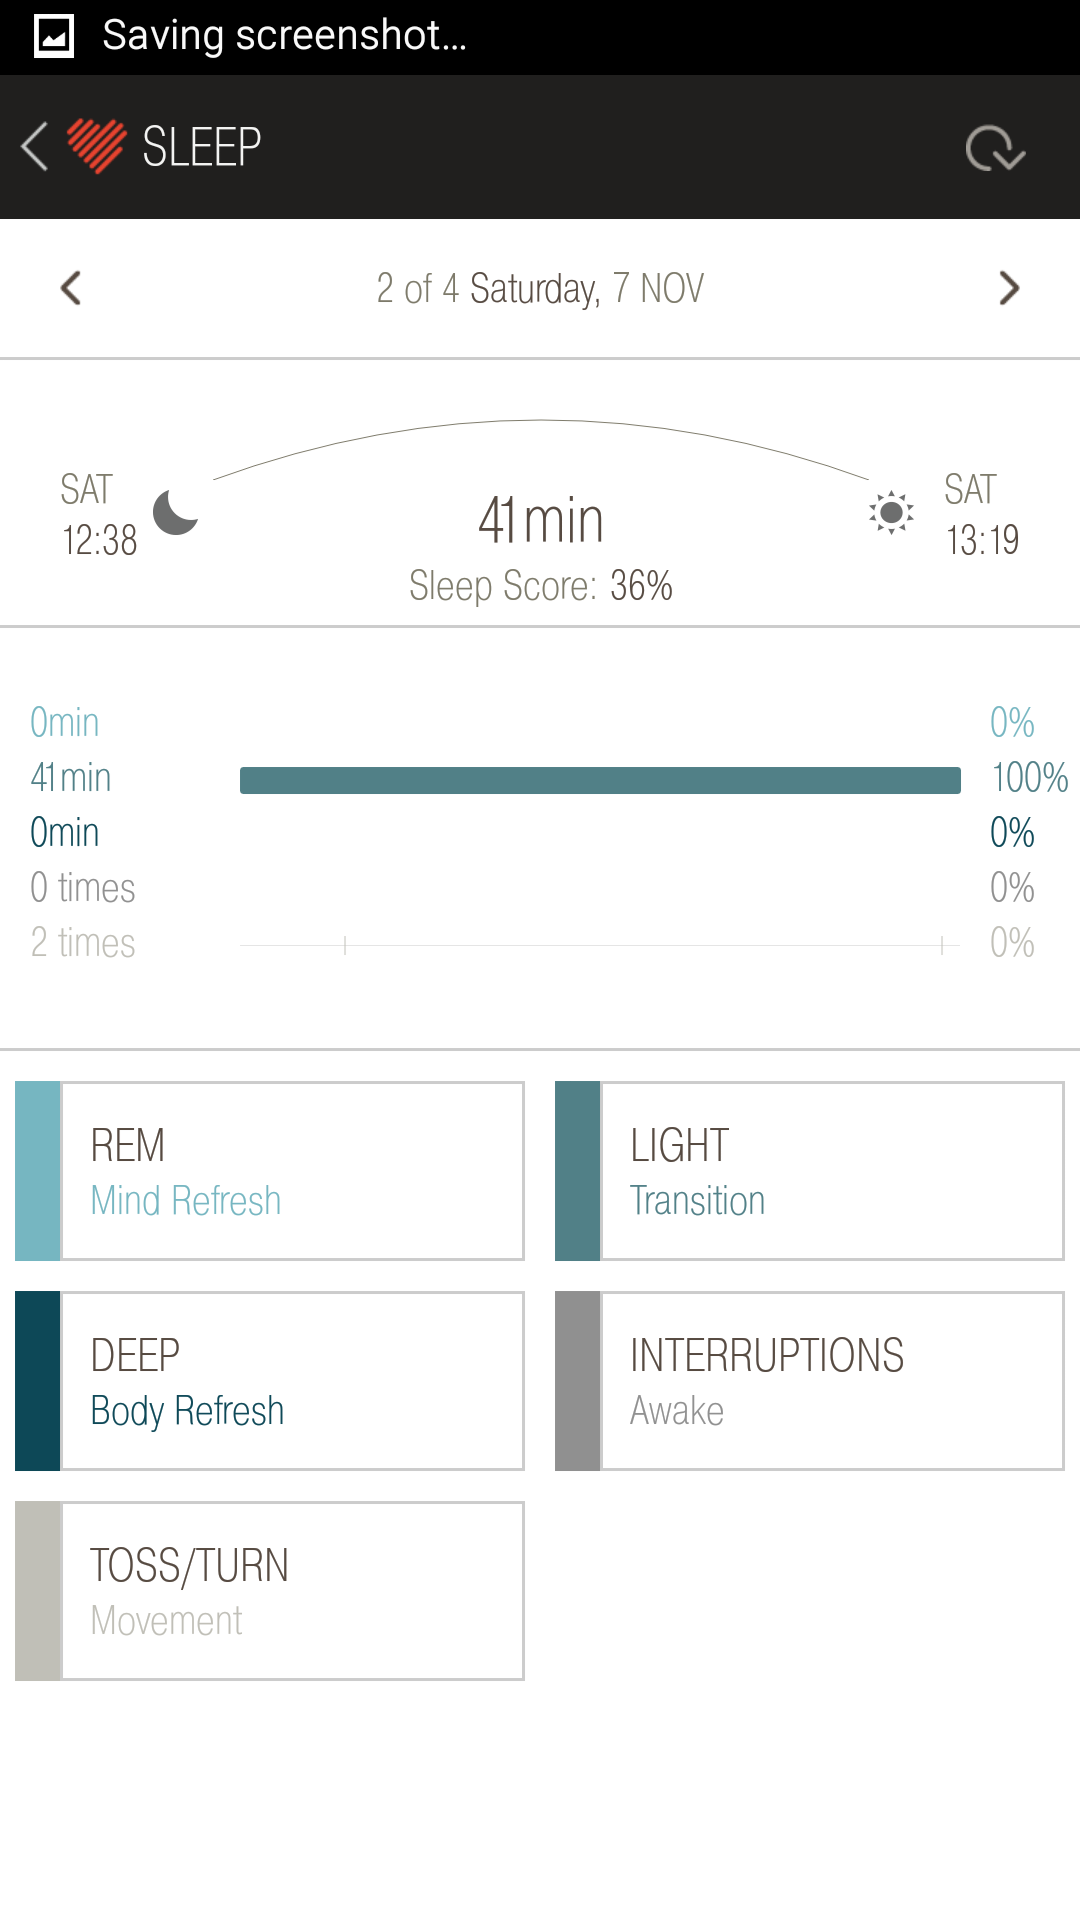
\includegraphics[width=\textwidth]{07-11-15-2.png}
    \end{subfigure}
\caption{Friday night I was working at our student bar - and then I needed to get up and help my boyfriend move to his new apartment. While him and his dad was picking up the trailer, I fell asleep at the couch - so everything looks right here, except from the unknown ~4 minutes on the first one. The app says it can be because the watch is placed wrongly or I was sleeping weird... }
\end{figure}

\newpage

\begin{figure}[H]
    \begin{subfigure}[b]{0.5\textwidth}
        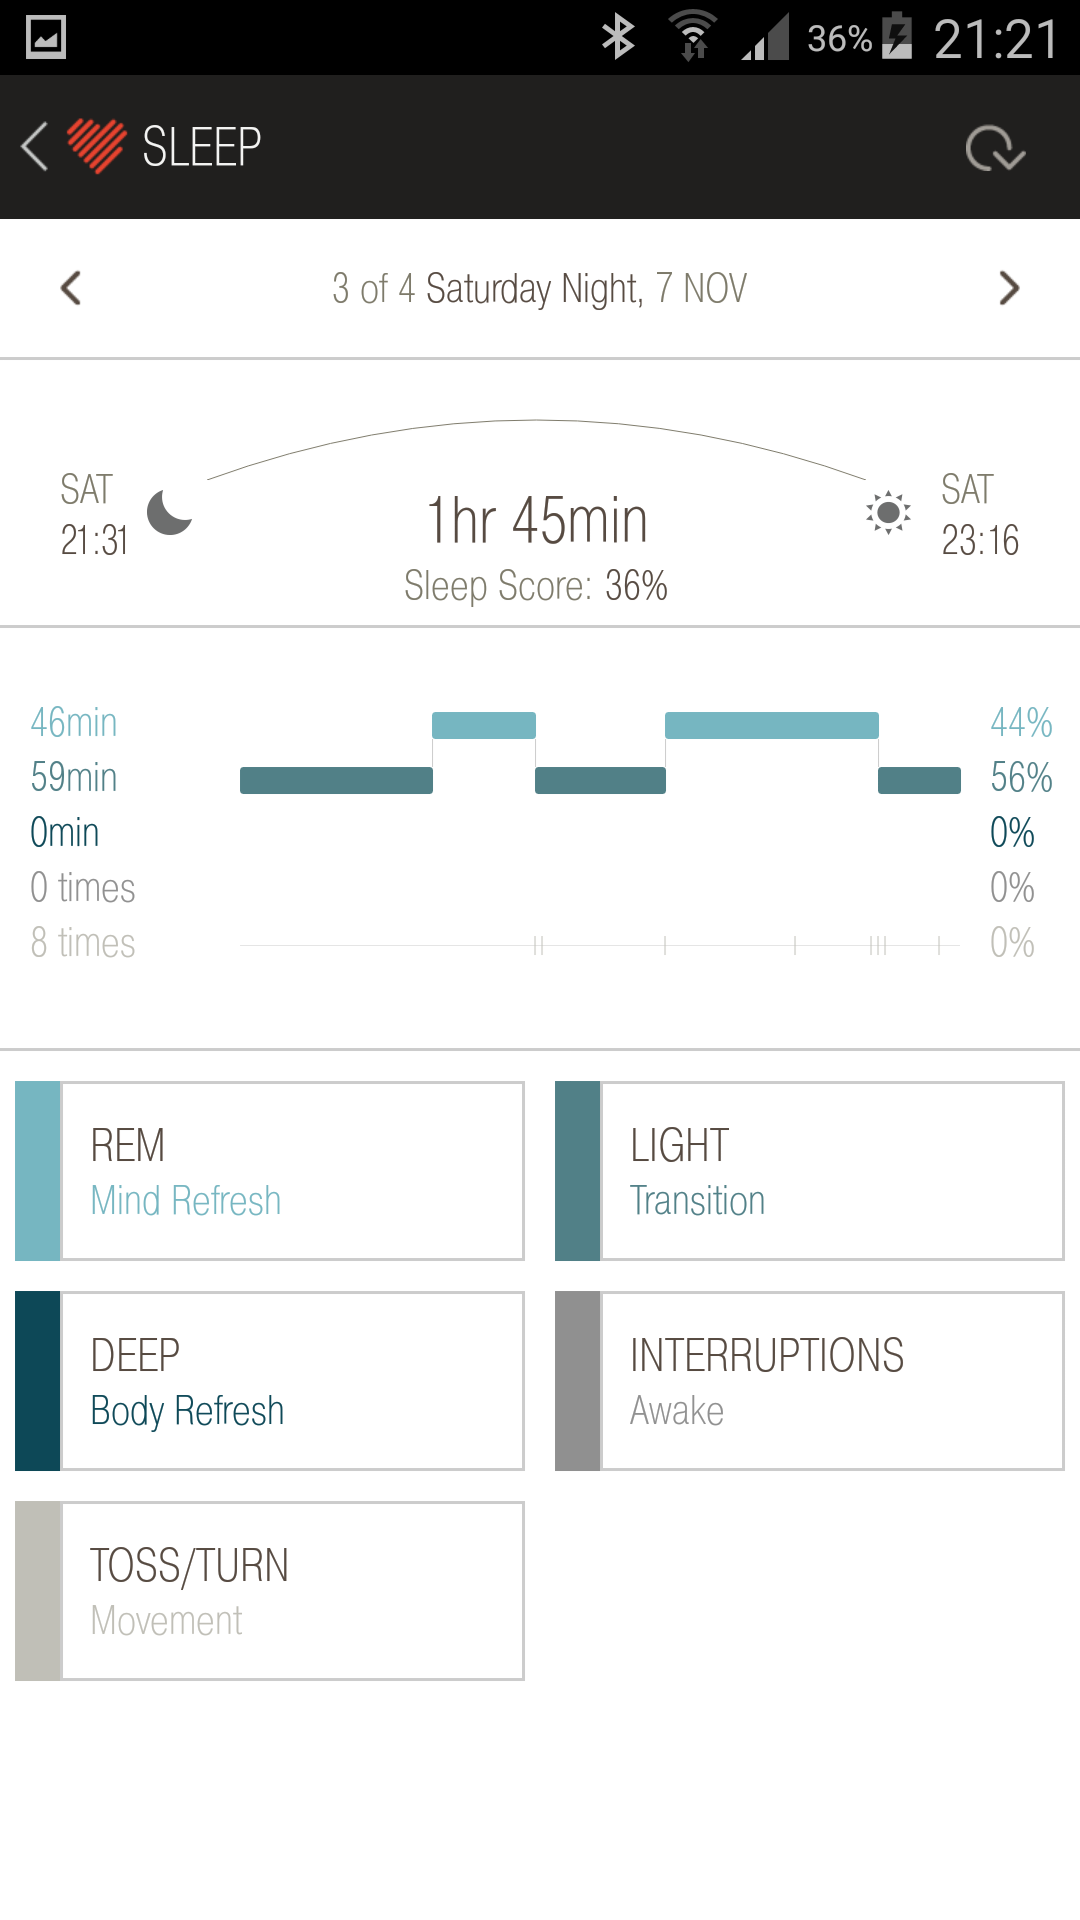
\includegraphics[width=\textwidth]{07-11-15-3.png}
     \end{subfigure}
    ~ %add desired spacing between images, e. g. ~, \quad, \qquad, \hfill etc. 
      %(or a blank line to force the subfigure onto a new line)
    \begin{subfigure}[b]{0.5\textwidth}
        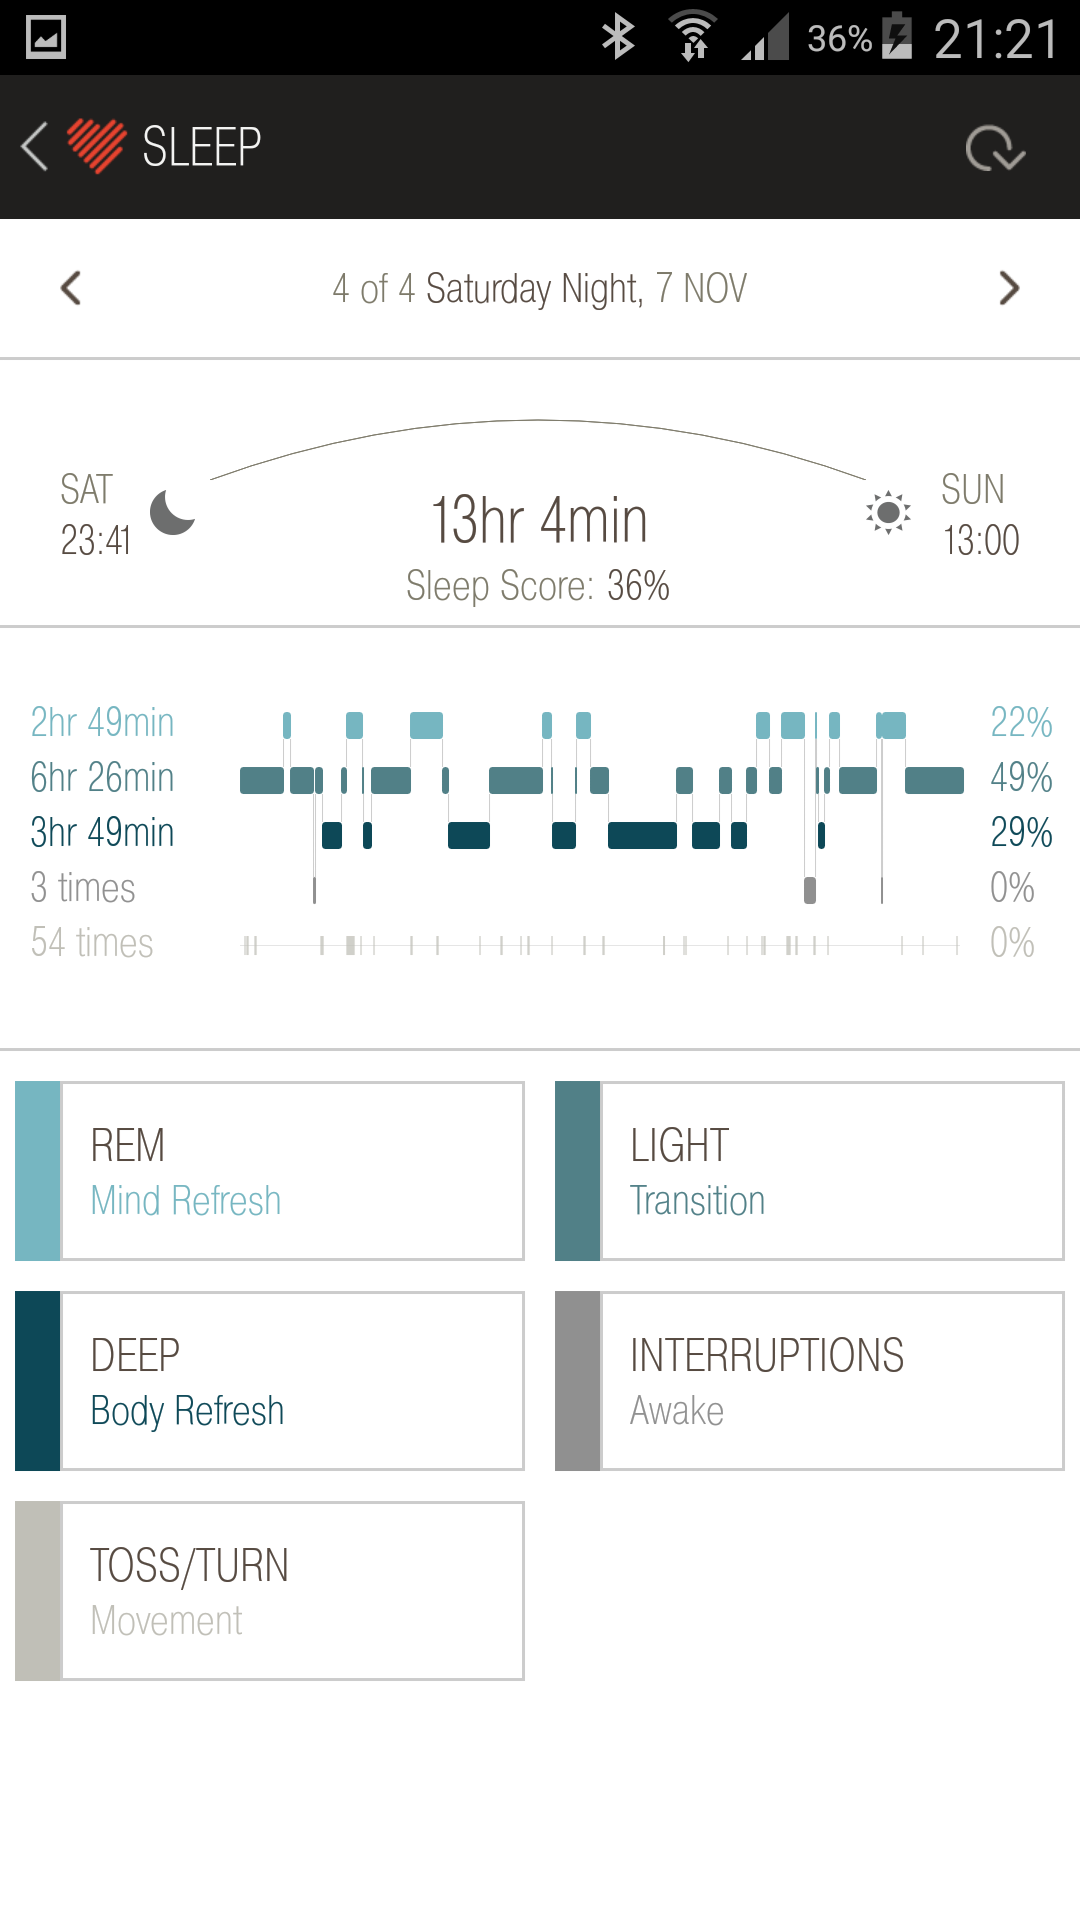
\includegraphics[width=\textwidth]{07-11-15-4.png}
    \end{subfigure}
\caption{After moving my boyfriend and his stuff, we where pretty tired and went to bed early. As you can see, there is a 25 minutes gap from 23:16 to 23:41 - I was having fun with my boyfriend. ;o)}
\end{figure}

\newpage

\begin{figure}[H]
    \begin{subfigure}[b]{0.5\textwidth}
        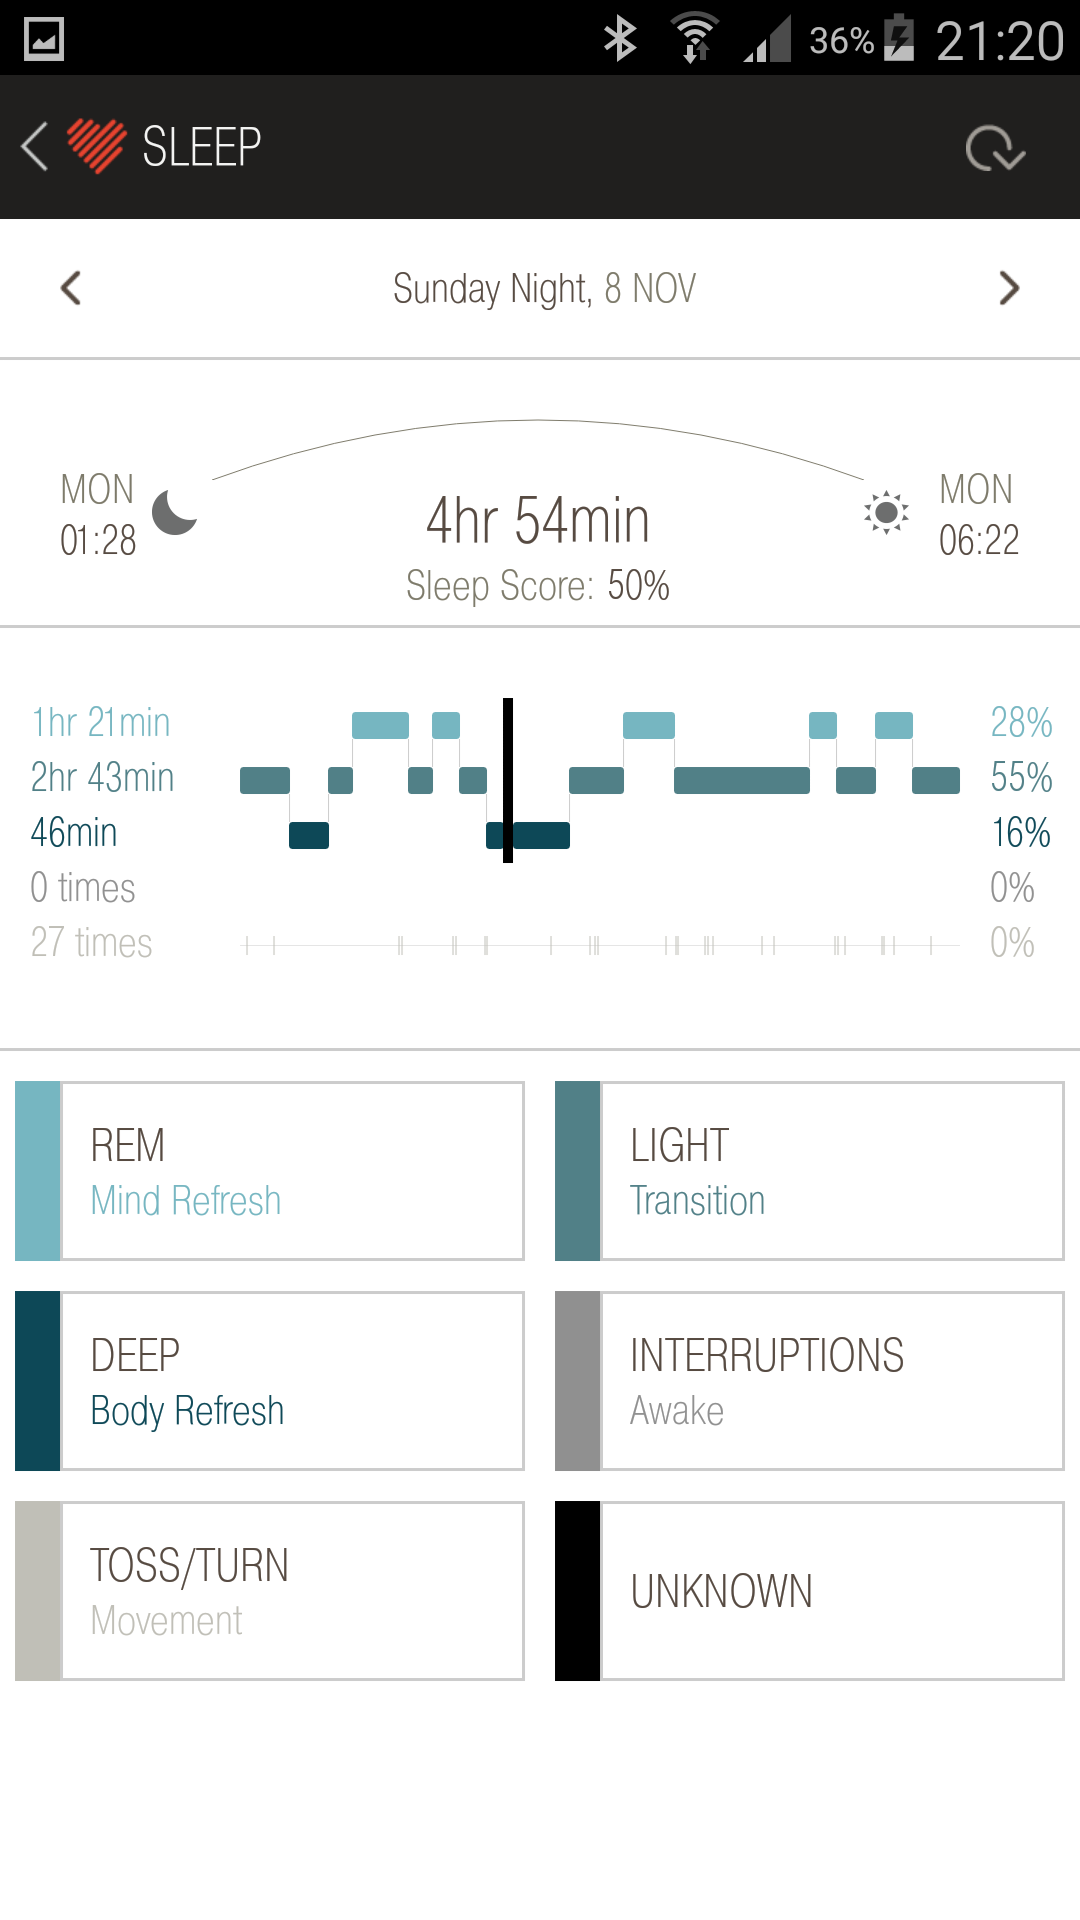
\includegraphics[width=\textwidth]{08-11-15.png}
     \end{subfigure}
    ~ %add desired spacing between images, e. g. ~, \quad, \qquad, \hfill etc. 
      %(or a blank line to force the subfigure onto a new line)
    \begin{subfigure}[b]{0.5\textwidth}
        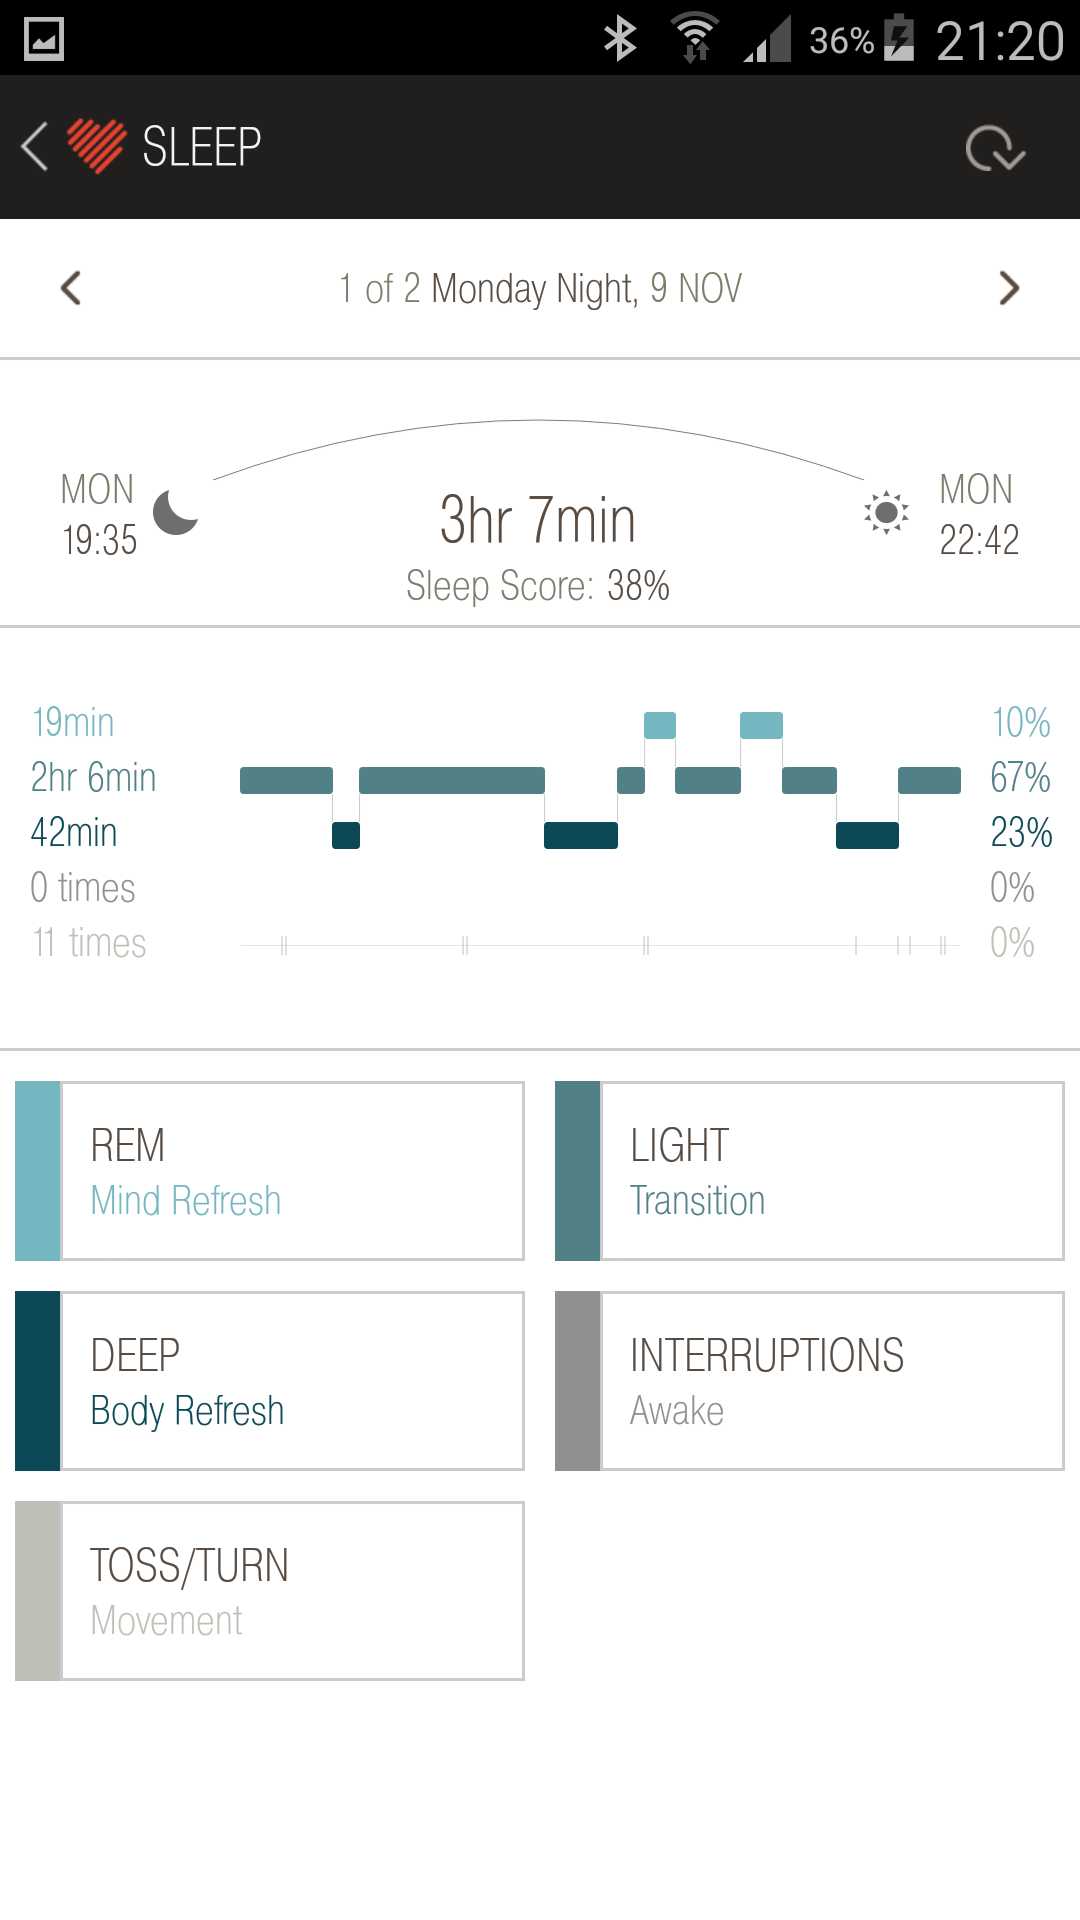
\includegraphics[width=\textwidth]{09-11-15-1.png}
    \end{subfigure}
\caption{Once again I went to bed way to late - which is also why I might have looked pretty tired Monday morning for our meeting Kate. :) Also - I once again have that 4-5 minutes period where no one knows what is happening. Due to the lack of sleep in the night, I fell asleep at my couch when I got home. }
\end{figure}

\newpage

\begin{figure}[H]
    \begin{subfigure}[b]{0.5\textwidth}
        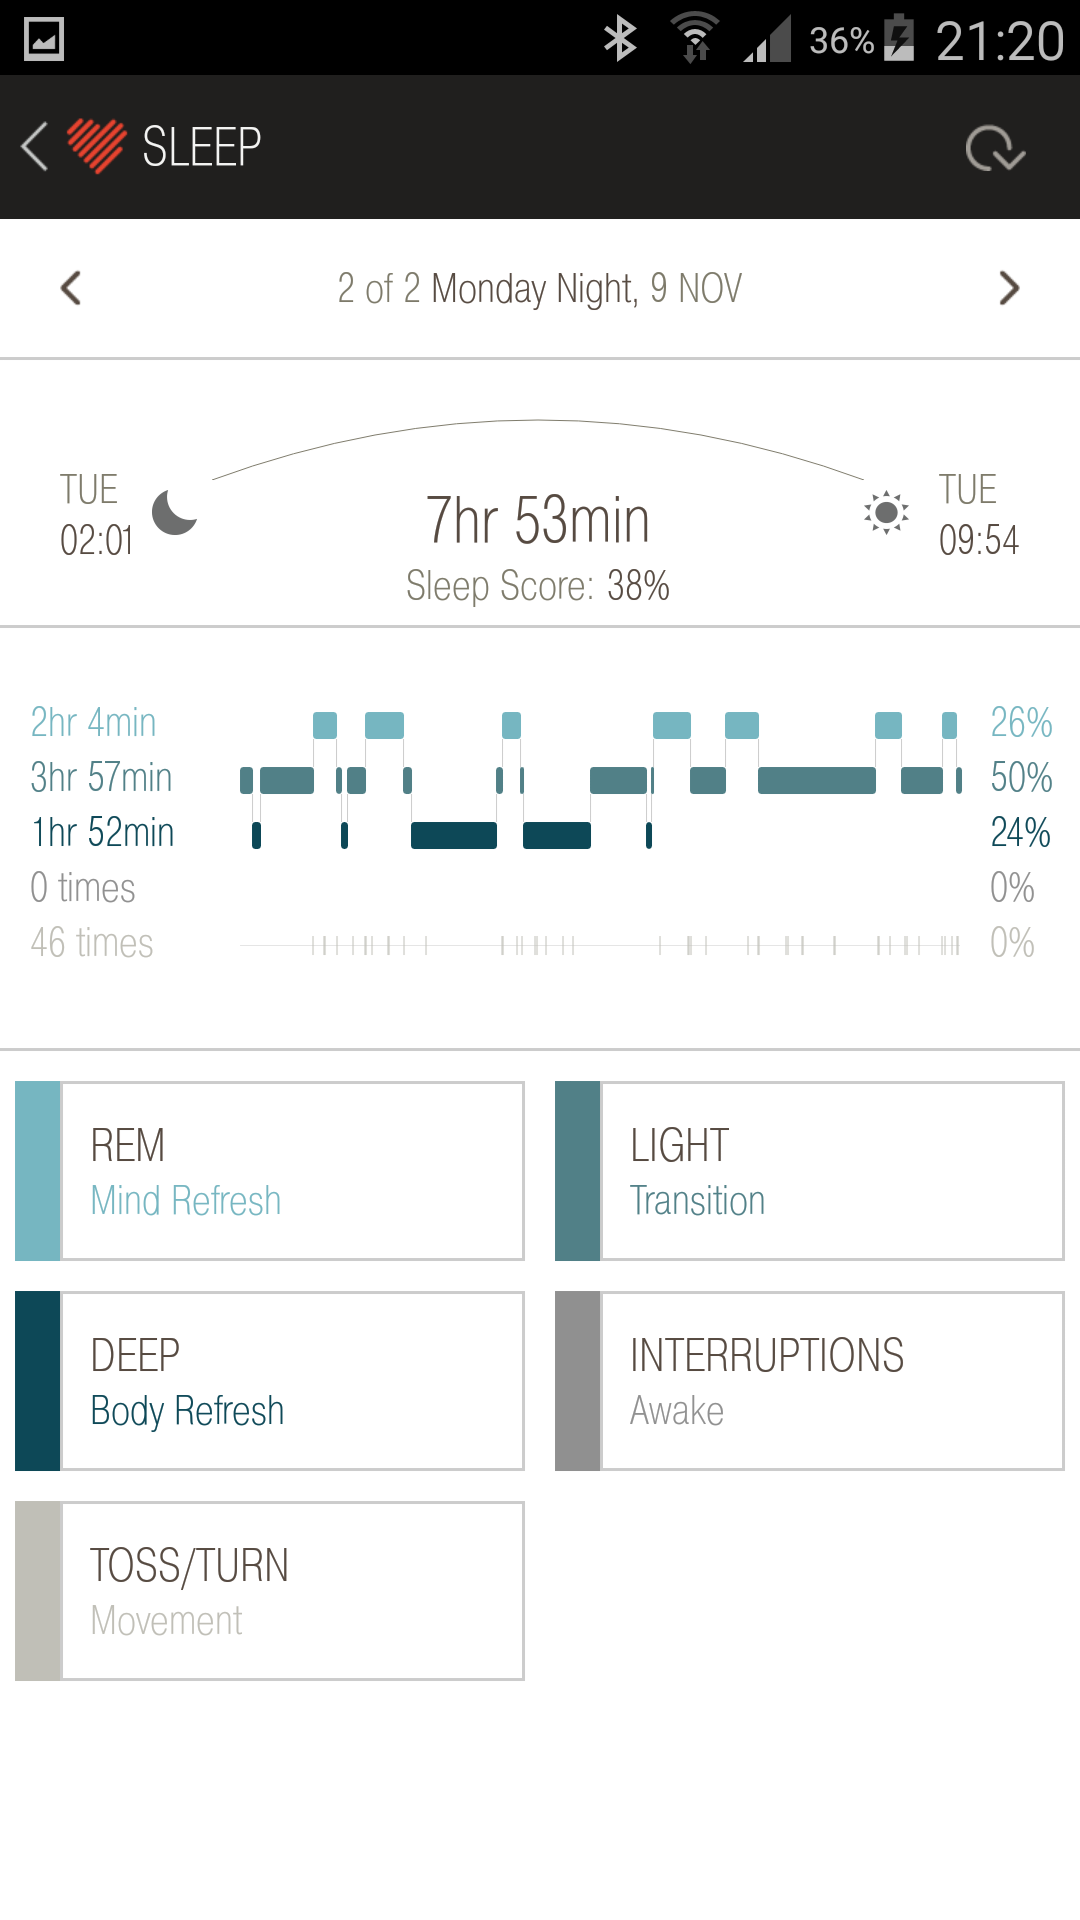
\includegraphics[width=\textwidth]{09-11-15-2.png}
     \end{subfigure}
    ~ %add desired spacing between images, e. g. ~, \quad, \qquad, \hfill etc. 
      %(or a blank line to force the subfigure onto a new line)
    \begin{subfigure}[b]{0.5\textwidth}
        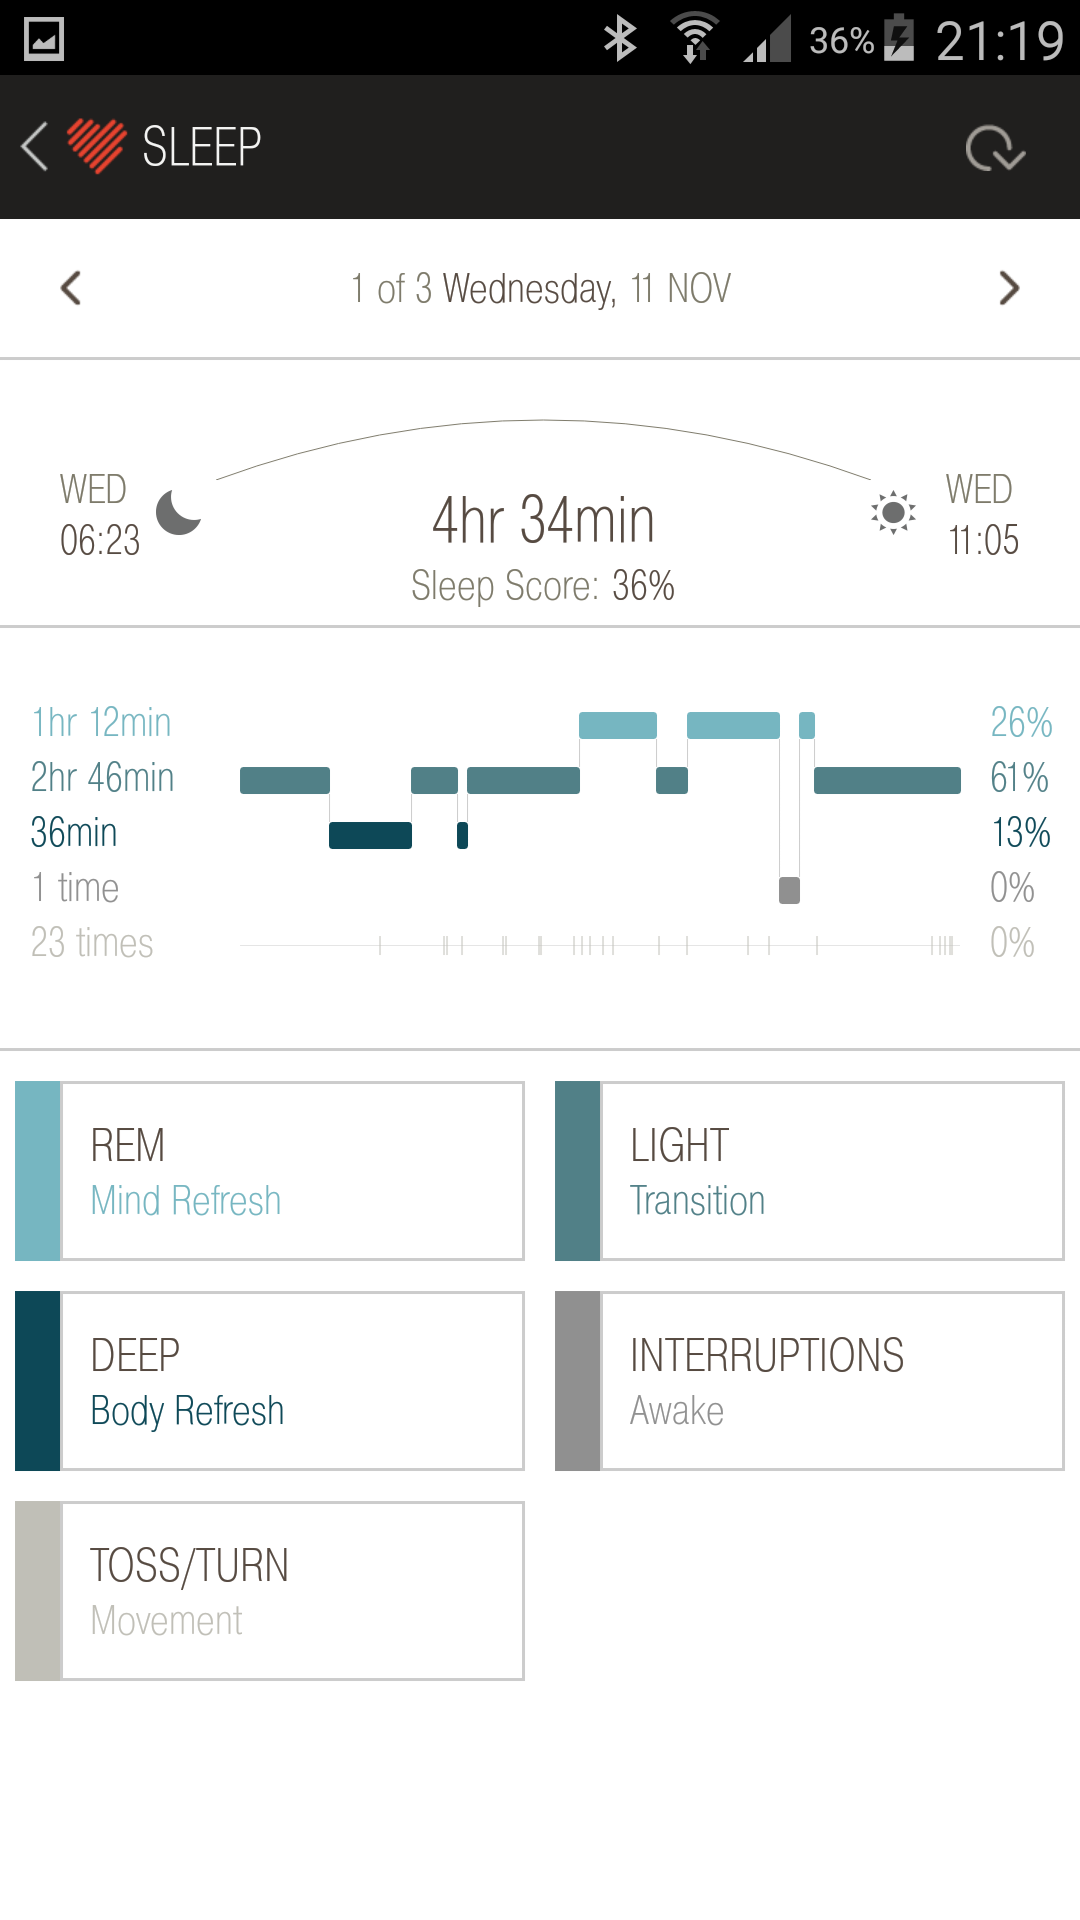
\includegraphics[width=\textwidth]{11-11-15-1.png}
    \end{subfigure}
\caption{A somewhat normal night of sleep! But I messed that up by going to a board meeting at the student bar, where we ended up having a party afterwards... That resulted in me only getting 4 hours and 34 minutes of sleep before I had to meet with some of my participants for the project.}
\end{figure}

\newpage

\begin{figure}[H]
    \begin{subfigure}[b]{0.5\textwidth}
        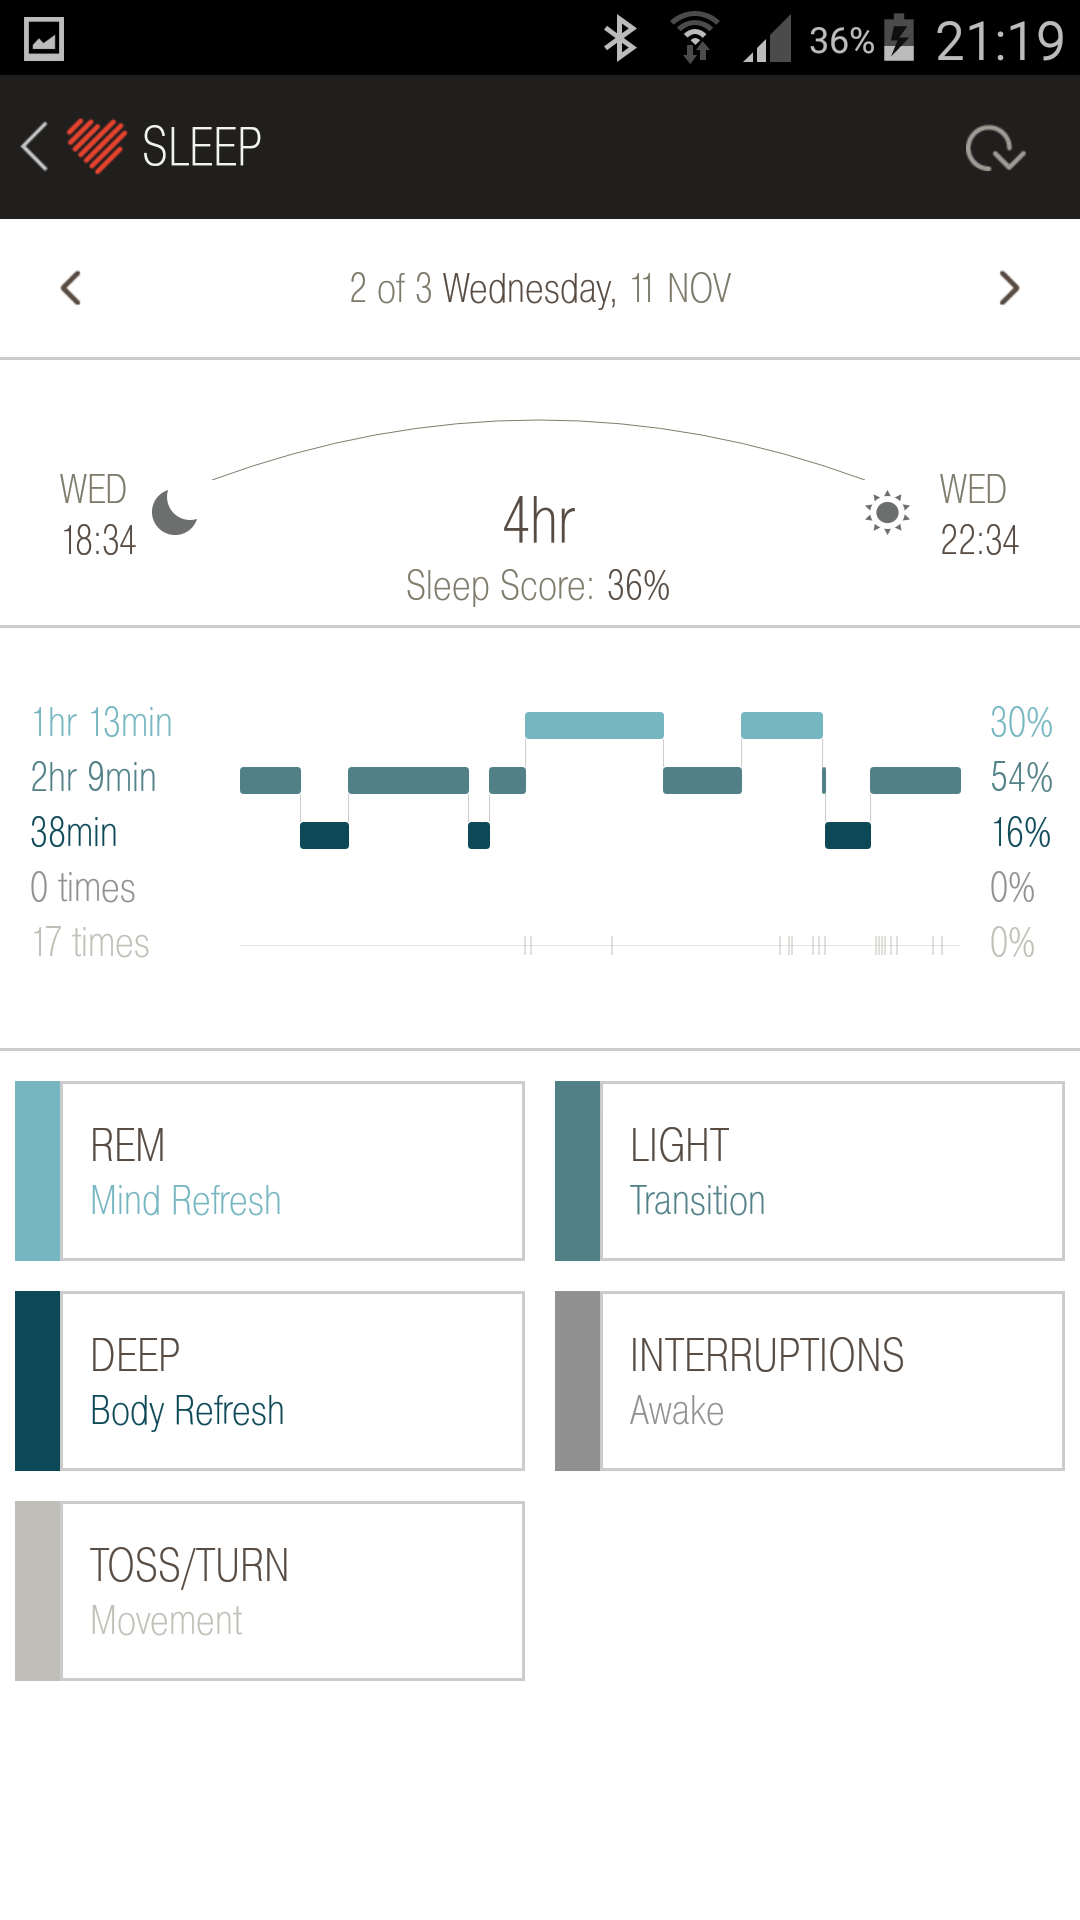
\includegraphics[width=\textwidth]{11-11-15-2.png}
     \end{subfigure}
    ~ %add desired spacing between images, e. g. ~, \quad, \qquad, \hfill etc. 
      %(or a blank line to force the subfigure onto a new line)
    \begin{subfigure}[b]{0.5\textwidth}
        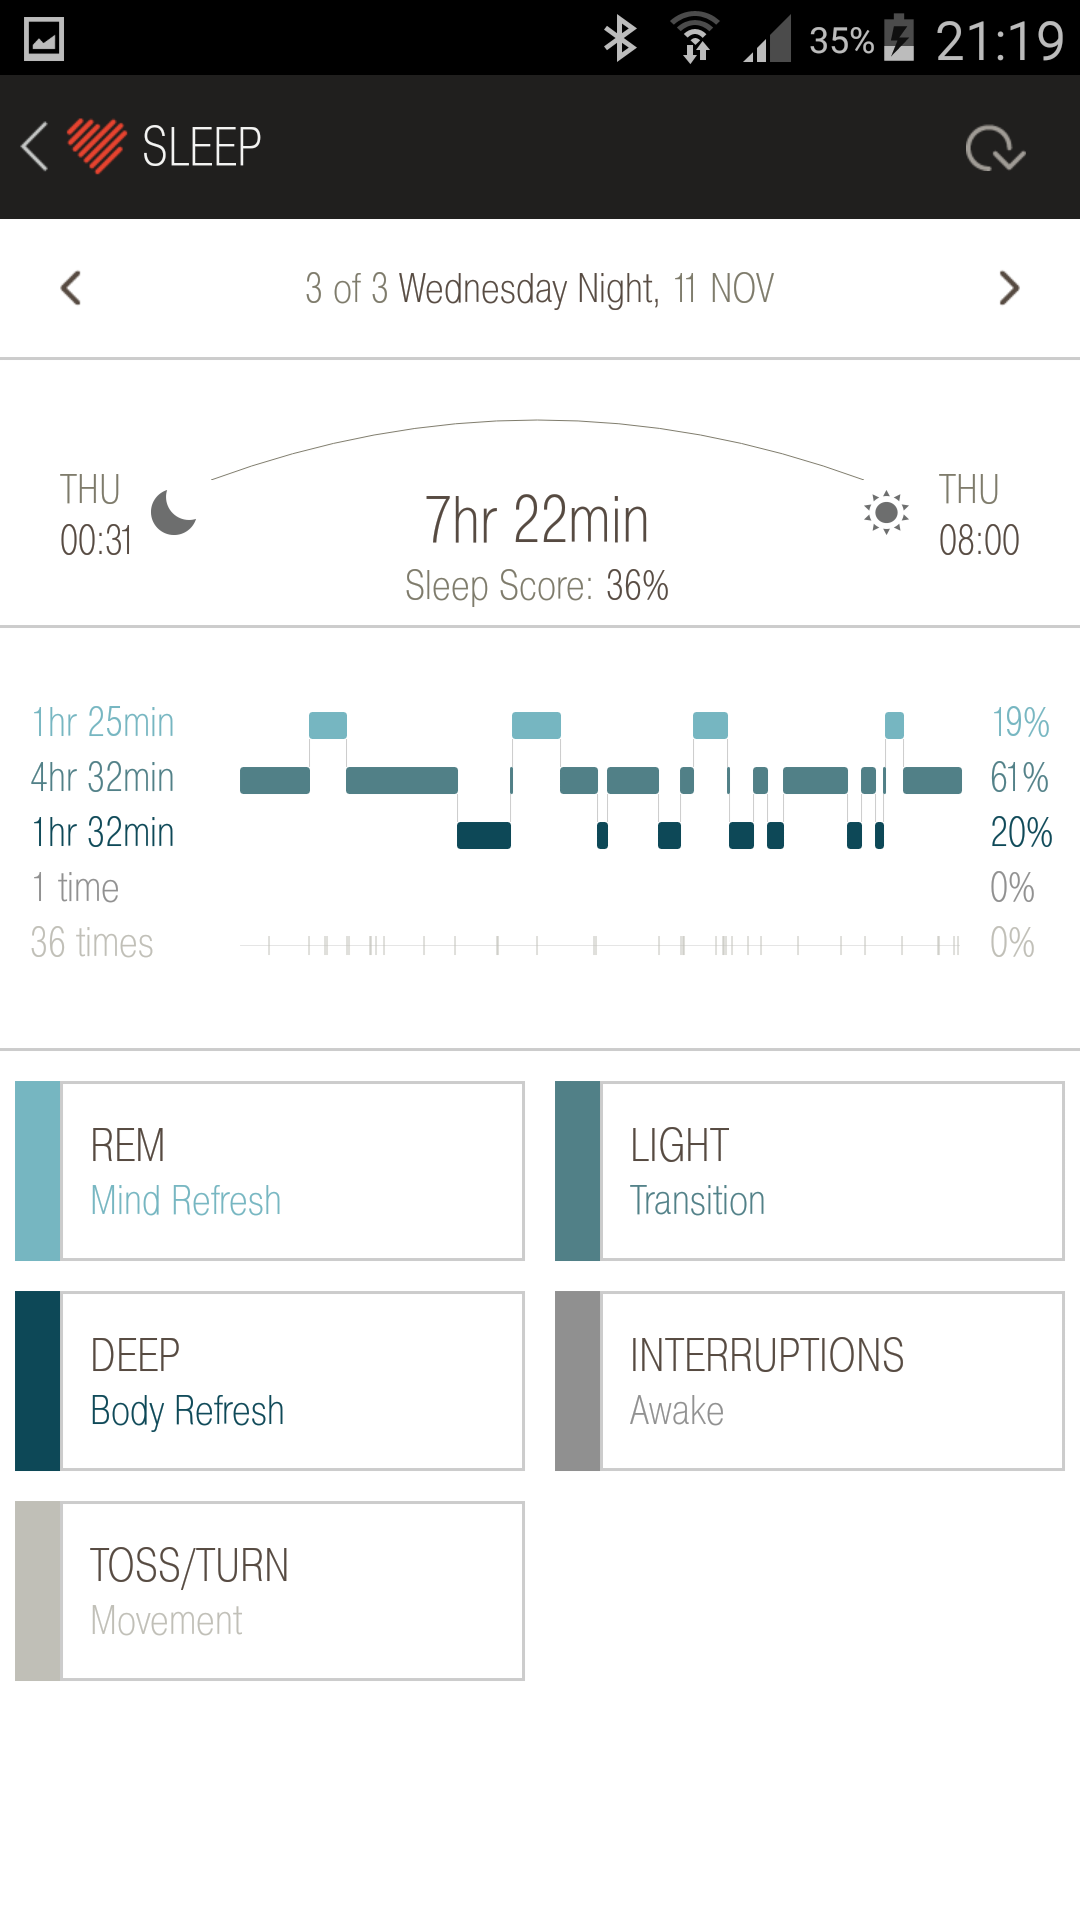
\includegraphics[width=\textwidth]{11-11-15-3.png}
    \end{subfigure}
\caption{Due to the lack of sleep in the night, I again fell asleep on the couch - this time for 4 hours. I was still sleepy after that, and of course my head was still not relaxed enough after my exam, so I went to bed and slept for ~7 hours more.}
\end{figure}

\newpage

\begin{figure}[H]
    \begin{subfigure}[b]{0.5\textwidth}
        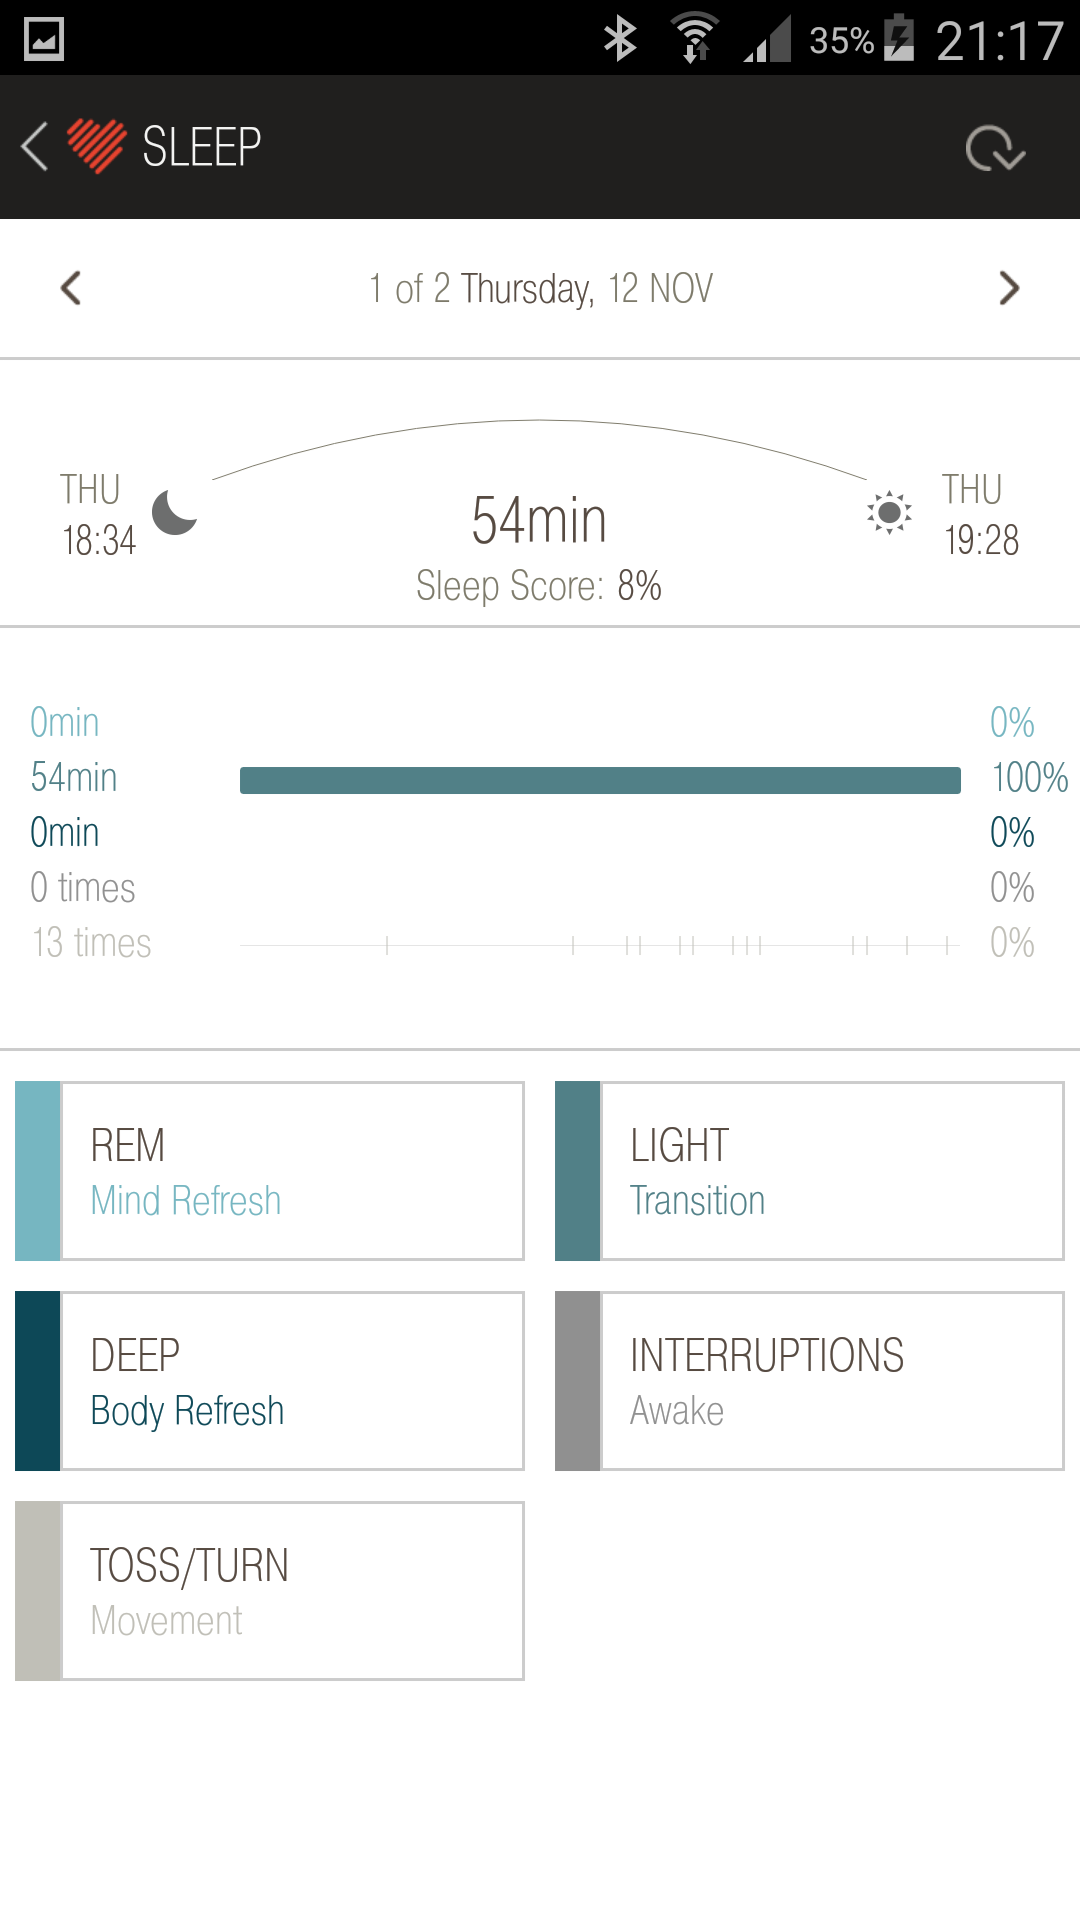
\includegraphics[width=\textwidth]{12-11-15-1.png}
     \end{subfigure}
    ~ %add desired spacing between images, e. g. ~, \quad, \qquad, \hfill etc. 
      %(or a blank line to force the subfigure onto a new line)
    \begin{subfigure}[b]{0.5\textwidth}
        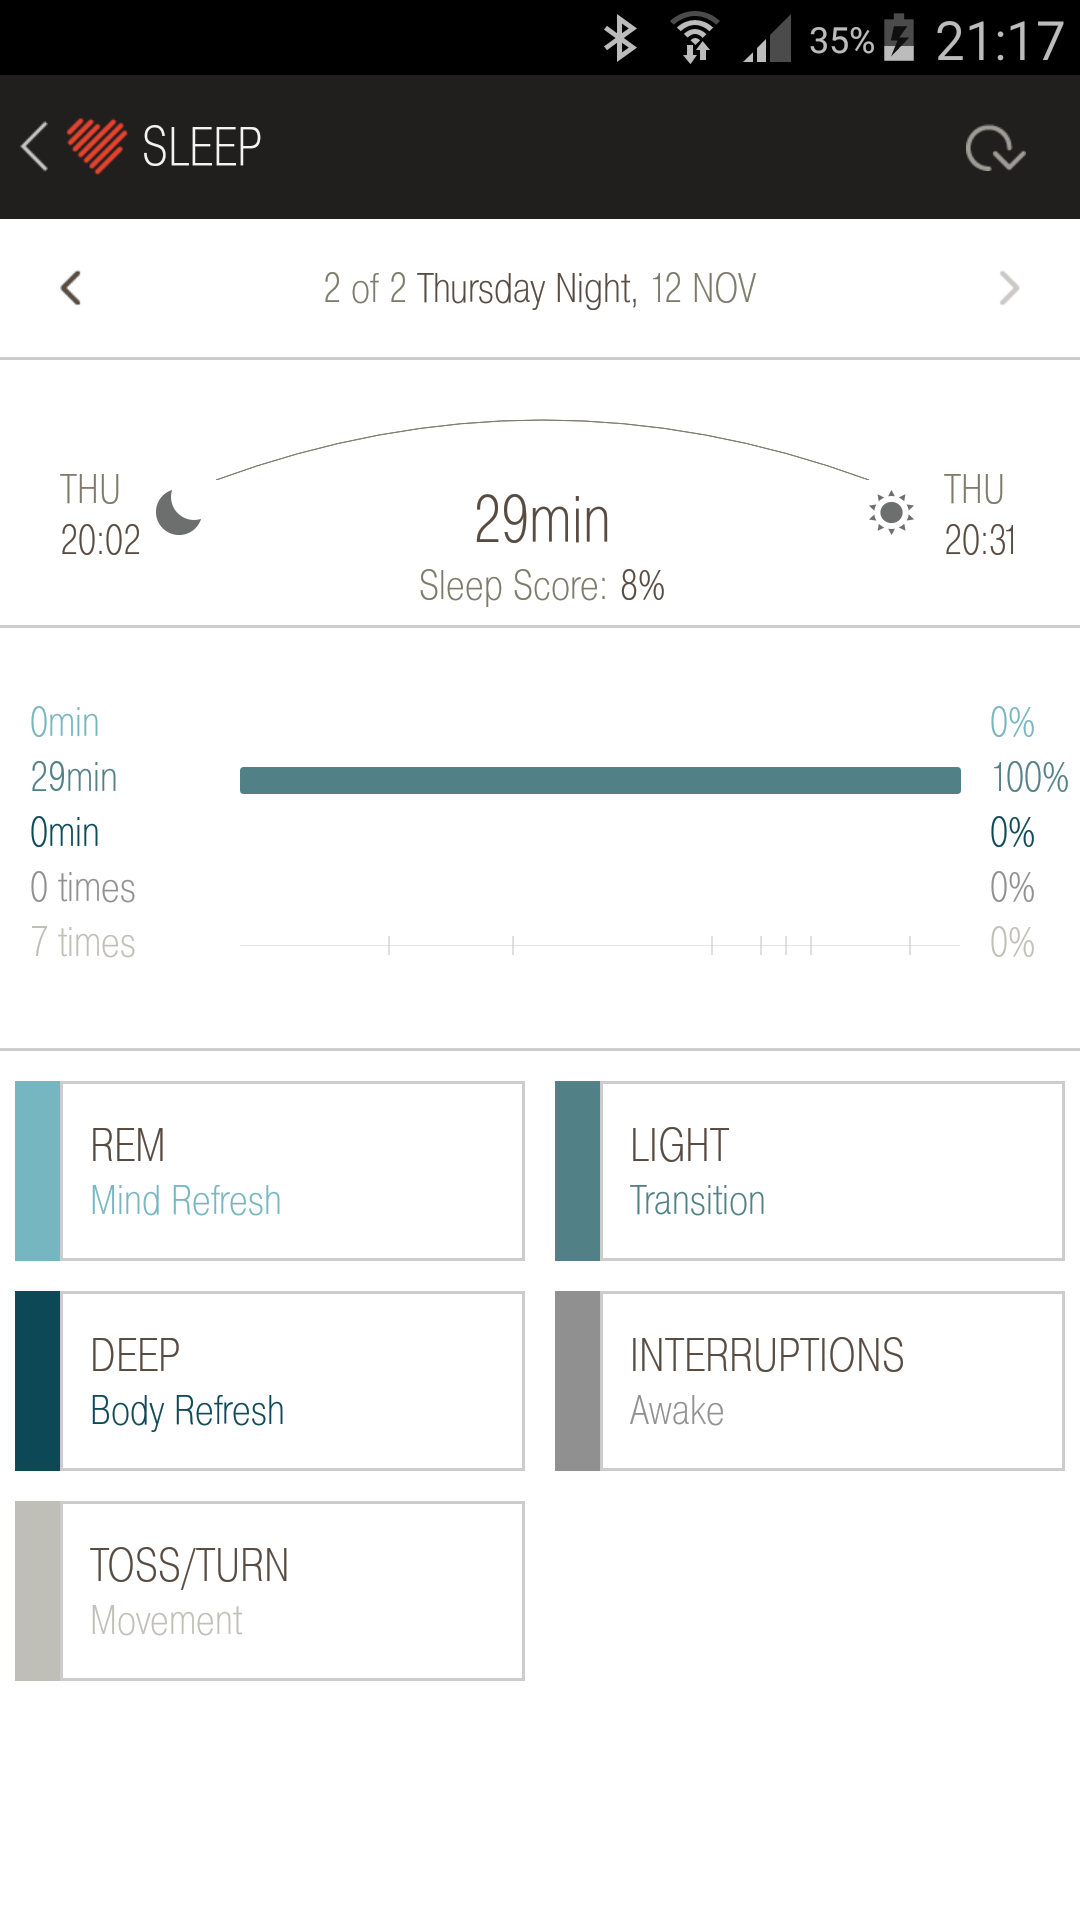
\includegraphics[width=\textwidth]{12-11-15-2.png}
    \end{subfigure}
\caption{These two I have no clue about - or - I do, it is me lying on my couch working on setting up the Android phone as my primary phone, so I can see my own data also. Apparently I am working pretty still, because the watch thought I was asleep. This is the second time, I have falls positives, and this time two in a day. }
\end{figure}



%-----------------------------------------------------------------------------
\end{document}